\documentclass{beamer} %NEW
\usetheme{Madrid}
%\usepackage{times,a4wide} %OUT
\usepackage{verbatim}
\usepackage{graphicx}
\usepackage{amssymb}
%\usepackage{html}
\usepackage{epstopdf}
\DeclareGraphicsRule{.tif}{png}{.png}{`convert #1 `dirname #1`/`basename #1 .tif`.png}
\usepackage[round]{natbib}

\title{My Project Report}
\author{A. Goldsmiths-Student\\Supervisor: Dr Ann Academic}
\date{\today}                                           % Activate to display a given date or no date

\begin{document}
\def\newblock{\hskip .11em plus .33em minus .07em}

\maketitle
\def\thepage{\roman{page}}
\begin{frame}
\frametitle{Abstract}
This is the abstract of my report.
\end{frame}
\newpage

\begin{comment}
\chapter*{Acknowledgements}
I am hugely grateful to the people who helped me\ldots
%\tableofcontents
%\listoffigures
%\listoftables
\end{comment}
%\chapter{Introduction}
\def\thepage{\arabic{page}}
\setcounter{page}{1}

\begin{frame}
\frametitle{The problem I am solving}
These titles should not appear word for word in your report. They are guidelines as to the meaning of the titles that you should insert. There does need to be a chapter or section for each of these headings, though, regardless of exactly what you call them, and you may want to add more, depending on what you need to say.


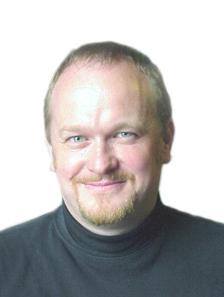
\includegraphics[height=60mm]{mugshot.jpg}

Part of the learning objectives of level 3 (which is where you are now) is the exercise of critical judgement; it is up to you to judge critically what appropriate titles and wordings for your report are, based on academic reports you have read during your course of study.

\end{frame}

\begin{frame}
  \frametitle{Why my problem is interesting}
 \begin{itemize}
 \item<1->{Schema theory was introduced in the 1950s by a Russian Mathematician, 
 Ianov. It was seen as a way of proving the correctness of compiler optimisations.}
 
 \item<2->{Schemas are an abstract way of representing classes of programs
 with identical structure.}

 
\end{itemize}
\end{frame}  

\begin{frame}

\frametitle{In this talk:}
\uncover<1->{\begin{quote}
\citet{ArticleA} argue that nothing is true. You use this if you need to make the authors part of your sentence. Look at the {\tt .tex} file to see how this is done.
\end{quote}}

\uncover<2->{
The second is as follows:
\begin{quote}
It has been argued that nothing is true \citep{ArticleA}. You use this if you don't mention the authors in your sentence. Look at the {\tt .tex} file to see how this is done.
\end{quote}
When you do this, you must have a definition for each item in your {\tt DoCReport.bib} file. There is an example to help you, for journal articles \citep{ArticleA}, books \citep{BookB}, chapters in collection books \citep{CollectedC}, and miscellaneous things like web sites \citep{MiscD}. You can make up the keys for these things (that is, {\tt ArticleA}, {\it etc.}); you just need to make sure that each is unique. It doesn't matter what order to place the entries in the {\tt .bib} file.
}

\uncover<3->{
If you compare the entries in the {\tt .bib} file, you'll see that each is
rendered differently into a bibliography entry at the back of the formatted
report. LaTeX and BibTeX handle this correctly on your behalf -- but make sure
you read error messages and act on them, because the software can't correct any
errors you make!
}
\end{frame}

\begin{frame}
\frametitle{Help with \LaTeX}
You can get help with \LaTeX and BibTex from {\tt http://www.math.harvard.edu/texman/} \cite{KuhnScottAndreev2008}, and from 

\htmladdnormallink{http://en.wikibooks.org/wiki/LaTeX}{http://en.wikibooks.org/wiki/LaTeX}.
\end{frame}

\begin{frame}
\frametitle{An important thing to note!!}

\LaTeX deals carefully with all the forward and backward referencing in your document ({\it e.g.,} tables of contents, {\it etc.}). This means that you sometimes need to run it as many as three times before all the inter-dependencies are sorted out. Make sure you read the output of the program, which will tell you when you need to run it again.
\end{frame}

\begin{frame}
\begin{center}
\fbox{
This text is part of a figure. It is centred (note the American spelling!).}
\vspace{.5in}

Latex will put the figure at the place most appropriate for it, \\according to publishing convention, automatically.
\end{center}
{This is how you make a figure in your document.}
\end{frame}

\begin{frame}

\begin{table}
\begin{center}
\begin{tabular}{|cc|c|}
\hline
Part 1 & Part 2 & Part 3\\\hline
Result A & Result B & Total \\\hline
\end{tabular}
\end{center}
\caption{This is how you make a table in your document.}
\end{table}
\end{frame}

\section{Background}
\section{The Problem being solved}
\subsection{And various sections on each piece of background}
\section{The Science and Technology needed to solve it}
\subsection{In various sections, describing the technological tools you'll use}

\begin{frame}
\frametitle{Project Description}
   {Textual Description of what you have built}
\end{frame}

\begin{frame}
\frametitle{Block Diagram}
\end{frame}

\begin{frame}
\frametitle{Work Plan}
Describe the work plan you proposed in your second deliverable and assess whether you stuck to it.
\end{frame}


\chapter{System Evaluation}
\section{How my system/software can be tested}
\section{The results of testing my system/software}
\section{How I might improve my project based on this evaluation}

\chapter{Summary and Conclusions}
\section{Summary of the Project}
\subsection{Goals}
The project aimed to\ldots
\subsection{Outcomes}
The project achieved\ldots
\section{Conclusions Drawn from the Project}
This was a fabulous/good/bad/terrible way to address this task. Here's why\ldots

\chapter{Project Self-Evaluation}
\section{Introduction}
In this chapter, you reflect on what you did in your project and how well you did it.
\section{Project outcomes}
Did you meet the outcomes you said you would? If not, why not? How could you have done better?
\section{Project planning}
Did your planning work well? How could you improve it?
\section{Self-evaluation}
What you learned about yourself in doing this project.

\bibliographystyle{apalike}
\bibliography{DoCReport}

\end{document}  
